\documentclass[10pt,a4paper]{article}

\usepackage[margin=2.0cm]{geometry}
\usepackage[T1]{fontenc}
\usepackage[utf8]{inputenc}
\usepackage{lmodern}
\usepackage{amsmath,amssymb}
\usepackage{booktabs}
\usepackage{graphicx}
\usepackage{algorithm}
\usepackage{algpseudocode}
\usepackage[hidelinks]{hyperref}
\usepackage[noabbrev]{cleveref}

\emergencystretch=2em
\setlength{\parskip}{0.12em}
\setlength{\parindent}{1.05em}
\setlength{\floatsep}{8pt plus 2pt minus 2pt}
\setlength{\textfloatsep}{10pt plus 2pt minus 2pt}
\setlength{\intextsep}{8pt plus 2pt minus 2pt}
\setlength{\abovecaptionskip}{4pt}
\setlength{\belowcaptionskip}{1pt}
\hypersetup{%
  pdftitle={Thermodynamically Consistent 1D Superelastic NiTi Constitutive Modeling, Inverse Identification, and Seismic-Carbon Trade-Offs in Diagrid Frames},
  pdfauthor={Syed Nafiz Reja Hasib}
}

\title{Thermodynamically Consistent 1D Superelastic NiTi Constitutive Modeling, Inverse Identification, and Seismic-Carbon Trade-Offs in Diagrid Frames}
\author{%
  Syed Nafiz Reja Hasib\\[0.2em]
  {\normalsize Independent Researcher;\quad
  BEng Civil Engineering, Southwest Petroleum University}\\[0.45em]
  {\normalsize
  \href{https://orcid.org/0009-0002-7162-7890}{orcid.org/0009-0002-7162-7890}
  \quad
  \href{https://github.com/syednafizreja/diagrid-seismic-opt}{github.com/syednafizreja/diagrid-seismic-opt}}%
}
\date{26 November 2026}

\begin{document}
\maketitle

\begin{abstract}
\noindent
Superelastic NiTi is often added to a frame to buy recentering. The inventory prices it at 28.0~kgCO$_2$e/kg, against 1.55~kgCO$_2$e/kg for steel, so recentering has to be read with peak drift and carbon. One isothermal return map is identified under noise and then used to set a paired diagrid comparison. The map has a signed martensite fraction, a monitored Helmholtz energy, and a piecewise algorithmic tangent. On the audited cycles the discrete dissipation stays above $-10^{-9}$~MPa, and the tangent matches a central difference to a relative error of $1.85\times 10^{-10}$. A PyTorch stand-in, trained at 3\% stress noise, recovers the six parameters to within 8\%. The worst miss is the transformation strain, at 7.28\%. The frame does not integrate the return map. An OpenSeesPy flag-shaped fuse takes the same stresses and the same transformation tangent. On 80 paired canopies and one synthetic $0.40g$ record, NiTi lowers the mean absolute residual roof drift from 0.0659\% to 0.0175\%. Mean peak roof drift rises from 1.788\% to 3.397\% on every geometry, and cradle-to-gate carbon rises by 620.9~kgCO$_2$e. Lifecycle intensity is higher on 66 of the 80 designs. Grouped cross-validation and NSGA-II give a 95\% upper-confidence false-safe rate of zero on 160 held-out rows. The certified fronts collapse to two spans.
\end{abstract}

\section{Introduction}
\label{sec:intro}

Residual drift decides whether a frame can be used after the ground motion stops. Superelastic NiTi can pull a fuse back towards its original length. DesRoches, McCormick, and Delemont tested wire and bar for that reason and found recentering, measured by residual strain, in both section sizes \cite{desroches2004}. The same tests found equivalent viscous damping typically below 7\%, and they found that cyclic strains above 6\% degrade both the damping and the recentering.

Carbon pulls the other way. The inventory in this study prices NiTi at 28.0~kgCO$_2$e/kg and structural steel at 1.55~kgCO$_2$e/kg. A fuse at that factor has to earn its place by the response it changes. If it recenters the roof and, on the same designs, raises peak drift and cradle-to-gate carbon, the recentering is not a free improvement.

The gap is between those two calculations. Auricchio and Sacco gave a one-dimensional superelastic return map with a consistent tangent, written so that austenite and martensite can have different moduli \cite{auricchio1997}. Coupon tests then showed what that kind of loop does to residual strain \cite{desroches2004}. Neither result is a frame analysis, and neither result is a carbon account. What is missing is one parameter set carried from the return map, through a noisy identification, into a paired structural comparison that reports residual drift, peak drift, and carbon together.

This preprint does that for one timber diagrid canopy: a curved roof on four branching steel columns, with two seismic fuses at each column. The structural model is OpenSeesPy \cite{zhu2018,mckenna2011} at a synthetic peak ground acceleration of $0.40g$. Three results follow.

\begin{enumerate}
  \item The isothermal return map, its algorithmic tangent, and a discrete dissipation check (\cref{sec:const}, \cref{fig:const}). The tangent agrees with a central difference to a relative error of $1.85\times 10^{-10}$. On the audited loops the dissipation stays above $-10^{-9}$~MPa.
  \item A PyTorch identification under 3\% stress noise (\cref{sec:inverse}, \cref{tab:inverse}, \cref{fig:inverse}). All six parameters fall inside an 8\% relative-error gate. The worst error is 7.28\% on the transformation strain. The 95\% bootstrap intervals do not cover every true value.
  \item The paired $0.40g$ comparison, then a grouped cross-validation Gaussian process and NSGA-II \cite{rasmussen2006,deb2002} (\cref{sec:frame}, \cref{tab:compare}, \cref{fig:seismic,fig:gp}). NiTi lowers the mean absolute residual drift from 0.0659\% to 0.0175\%. It raises the mean peak drift from 1.788\% to 3.397\% on all 80 geometries, and it raises mean cradle-to-gate carbon by 620.9~kgCO$_2$e.
\end{enumerate}

The thermodynamic wording in the title means the dissipation check in \cref{sec:diss}. The model has no temperature. The 80 geometries are a designed sample inside stated bounds, not a census of diagrid roofs.

\section{Constitutive formulation and algorithmic verification}
\label{sec:const}

Auricchio and Sacco integrated a one-dimensional superelastic model by a return map and gave the consistent tangent of that discrete problem \cite{auricchio1997}. Their martensite fraction lies in $[0,1]$, and the austenite and martensite moduli may differ. The model audited here keeps the return-map idea and drops both of those features. It uses one Young's modulus, a signed martensite fraction $z\in[-1,1]$, and no temperature. The equations below are the ones in the code. Units in this section are MPa and dimensionless strain.

\subsection{Parameters and monitored free energy}
\label{sec:params}

The default parameters are also the identification targets. Young's modulus is $E=40000$~MPa and the transformation strain is $\varepsilon_L=0.06$. The transformation stresses are $\sigma_{Ms}=380$~MPa, $\sigma_{Mf}=450$~MPa, $\sigma_{As}=180$~MPa, and $\sigma_{Af}=110$~MPa. The hardening moduli are therefore equal,
\begin{equation}
  H_f=\sigma_{Mf}-\sigma_{Ms}=70~\mathrm{MPa},
  \qquad
  H_r=\sigma_{As}-\sigma_{Af}=70~\mathrm{MPa}.
\end{equation}
A state with $|z_n|>1$ is rejected. Write $\xi=|z|$. The stored energy uses the averages
\begin{equation}
  \sigma_0=\tfrac12(\sigma_{Ms}+\sigma_{Af})=245~\mathrm{MPa},
  \qquad
  H_{eq}=\tfrac12(H_f+H_r)=70~\mathrm{MPa},
\end{equation}
and
\begin{equation}
  \label{eq:psi}
  \psi(\varepsilon,z)
  =\tfrac12 E\,(\varepsilon-\varepsilon_L z)^2
  +\varepsilon_L\Bigl(\sigma_0\,|z|+\tfrac12 H_{eq}\,z^2\Bigr).
\end{equation}
There is no entropy and no heat flux. The stress returned on every branch, $\sigma=E(\varepsilon-\varepsilon_L z)$, is the partial derivative of $\psi$ with respect to strain at fixed $z$. The evolution of $z$ is not obtained by minimising an incremental potential of $\psi$. The energy is evaluated after the update so that the discrete dissipation can be checked. It is a monitor.

\subsection{Trial stress and the return map}
\label{sec:return}

One step is closed form. There is no constitutive Newton iteration inside the stress update. The trial stress and the sign convention are
\begin{equation}
  \label{eq:trial}
  \sigma^{\mathrm{tr}}=E\,(\varepsilon_{n+1}-\varepsilon_L z_n),
  \qquad
  s^{\mathrm{tr}}=\mathrm{sign}_{+}(\sigma^{\mathrm{tr}}),
  \qquad
  s_n=\mathrm{sign}_{+}(z_n),
\end{equation}
with $\mathrm{sign}_{+}(0)=+1$. The forward and reverse thresholds depend on the current martensite magnitude $\xi_n=|z_n|$,
\begin{equation}
  \sigma_f(\xi)=\sigma_{Ms}+H_f\xi,
  \qquad
  \sigma_r(\xi)=\sigma_{Af}+H_r\xi.
\end{equation}
The two measures that open a branch are
\begin{equation}
  \Phi_f=|\sigma^{\mathrm{tr}}|-\sigma_f(\xi_n),
  \qquad
  \Phi_r=\sigma_r(\xi_n)-s_n\sigma^{\mathrm{tr}}.
\end{equation}
If $|z_n|>0$ and $\Phi_r>0$, the reverse increment is
\begin{equation}
  \label{eq:dr}
  \Delta\xi_r=\frac{\sigma_r(\xi_n)-s_n\sigma^{\mathrm{tr}}}{E\varepsilon_L+H_r}.
\end{equation}
When $\Delta\xi_r<\xi_n$ the update is $z_{n+1}=s_n(\xi_n-\Delta\xi_r)$. When $\Delta\xi_r\ge\xi_n$ the step clears the martensite, sets the trial from a clean austenite state, and continues, so a forward transformation can still occur in the same step. The forward branch is taken if $\xi_n<1$, $\Phi_f>0$, and either $z_n=0$ or $s^{\mathrm{tr}}=s_n$. Its increment is
\begin{equation}
  \label{eq:df}
  \Delta\xi_f=\frac{|\sigma^{\mathrm{tr}}|-\sigma_f(\xi_n)}{E\varepsilon_L+H_f}.
\end{equation}
If $\xi_n+\Delta\xi_f<1$ then $z_{n+1}=s^{\mathrm{tr}}(\xi_n+\Delta\xi_f)$. Otherwise the martensite saturates, $z_{n+1}=s^{\mathrm{tr}}$. Any other step is elastic, $z_{n+1}=z_n$. On every branch the stress is
\begin{equation}
  \label{eq:stress}
  \sigma=E\,(\varepsilon_{n+1}-\varepsilon_L z_{n+1}).
\end{equation}
\Cref{alg:return} is that control flow.

\begin{algorithm}[t]
\caption{Signed-martensite return map. One closed-form step.}
\label{alg:return}
\begin{algorithmic}[1]
\Require $\varepsilon_{n+1}$ and $z_n$ with $|z_n|\le 1$
\State $\xi_n\gets|z_n|$, and form $\sigma^{\mathrm{tr}}$, $s^{\mathrm{tr}}$, $s_n$, $\Phi_f$, $\Phi_r$ from the definitions above
\If{$|z_n|>0$ and $\Phi_r>0$}
  \State compute $\Delta\xi_r$ from \eqref{eq:dr}
  \If{$\Delta\xi_r<\xi_n$}
    \State $z_{n+1}\gets s_n(\xi_n-\Delta\xi_r)$
  \Else
    \State set $z_n\gets 0$, recompute the trial from austenite, and continue
  \EndIf
\EndIf
\If{$\xi_n<1$ and $\Phi_f>0$ and ($z_n=0$ or $s^{\mathrm{tr}}=s_n$)}
  \State compute $\Delta\xi_f$ from \eqref{eq:df}
  \If{$\xi_n+\Delta\xi_f<1$}
    \State $z_{n+1}\gets s^{\mathrm{tr}}(\xi_n+\Delta\xi_f)$
  \Else
    \State $z_{n+1}\gets s^{\mathrm{tr}}$
  \EndIf
\EndIf
\If{$z_{n+1}$ was not set}
  \State $z_{n+1}\gets z_n$
\EndIf
\State $\sigma\gets E(\varepsilon_{n+1}-\varepsilon_L z_{n+1})$
\end{algorithmic}
\end{algorithm}

\subsection{Algorithmic tangent}
\label{sec:tangent}

On an open regime the tangent is constant. Consider partial forward transformation, where $s^{\mathrm{tr}}$ does not change with strain and $\mathrm{d}\sigma^{\mathrm{tr}}/\mathrm{d}\varepsilon_{n+1}=E$. Differentiating \eqref{eq:df} gives
\begin{equation}
  \frac{\mathrm{d}\Delta\xi_f}{\mathrm{d}\varepsilon_{n+1}}
  =\frac{E}{E\varepsilon_L+H_f}.
\end{equation}
With $z_{n+1}=s^{\mathrm{tr}}(\xi_n+\Delta\xi_f)$ and $\sigma$ from \eqref{eq:stress},
\begin{equation}
  \label{eq:tangent}
  E_{\mathrm{alg}}
  =\frac{\mathrm{d}\sigma}{\mathrm{d}\varepsilon_{n+1}}
  =E\Biggl(1-\varepsilon_L\frac{E}{E\varepsilon_L+H_f}\Biggr)
  =\frac{E H_f}{E\varepsilon_L+H_f}.
\end{equation}
On the reverse branch the same reduction holds with $H_r$ in place of $H_f$. The sign works because $s_n^2=1$: the derivative of $z_{n+1}=s_n(\xi_n-\Delta\xi_r)$ brings one factor of $s_n$ from the chain rule on $\sigma^{\mathrm{tr}}$ and one factor from the update, and they cancel. With the default parameters $H_f=H_r$, so the two transformation tangents coincide,
\begin{equation}
  E_{\mathrm{alg}}=\frac{40000\times 70}{40000\times 0.06+70}
  =1133.603~\mathrm{MPa}.
\end{equation}
An elastic step, and a saturated step with $|z|=1$, both keep $E_{\mathrm{alg}}=E$.

The tangent was checked by central differences with step $h=10^{-7}$ at four states. The relative error $|(E_{\mathrm{alg}}-E_{\mathrm{num}})/E_{\mathrm{num}}|$ is $1.222\times 10^{-12}$ at $(\varepsilon,z_n)=(\pm 0.001,\,0)$ and $1.850\times 10^{-10}$ at $(\pm 0.025,\,\pm 0.2)$. The gate is $10^{-7}$. The worst value on this set is $1.850\times 10^{-10}$ (\cref{fig:const}).

A separate stress-driven Newton solve inverts $\sigma(\varepsilon)=\sigma_{\mathrm{target}}$ with the same tangent, $\varepsilon\leftarrow\varepsilon-r/E_{\mathrm{alg}}$, residual tolerance $10^{-12}$, and a limit of five iterations. From $z_n=0$ at $\sigma_{\mathrm{target}}=500$~MPa the solve takes four iterations and returns $\varepsilon=0.0725$, $z=1$, and $r=4.547\times 10^{-13}$. The state is saturated, and $E(0.0725-0.06)=500$~MPa, so the residual is roundoff on an exact elastic point past the end of the plateau.

\subsection{Discrete dissipation}
\label{sec:diss}

For an isothermal process with no heat flux, the Clausius--Duhem inequality reduces to a non-negative mechanical dissipation, $\sigma\dot\varepsilon-\dot\psi\ge 0$. The tests use the trapezoidal counterpart of that statement,
\begin{equation}
  \label{eq:diss}
  D
  =\tfrac12(\sigma_n+\sigma_{n+1})(\varepsilon_{n+1}-\varepsilon_n)
  -\bigl(\psi_{n+1}-\psi_n\bigr),
\end{equation}
and they require $D\ge -10^{-9}$~MPa. On strain histories $0.05\sin\phi$ the recomputed minima are $-2.02\times 10^{-15}$~MPa for five cycles at 5000 samples, $-1.70\times 10^{-15}$~MPa for five cycles at 5001 samples, and $-1.98\times 10^{-15}$~MPa for ten cycles at 5001 samples. All three sit above the gate. The small negative values are roundoff, not a sign change in the loop. Because $z$ is not a variational update of $\psi$, the check does not derive the return map. It only shows that, on these histories, the trapezoidal work stays above the gate once $\psi$ from \eqref{eq:psi} is subtracted. \Cref{fig:const} collects the loop, the tangent errors, and these minima.

\begin{figure}[t]
  \centering
  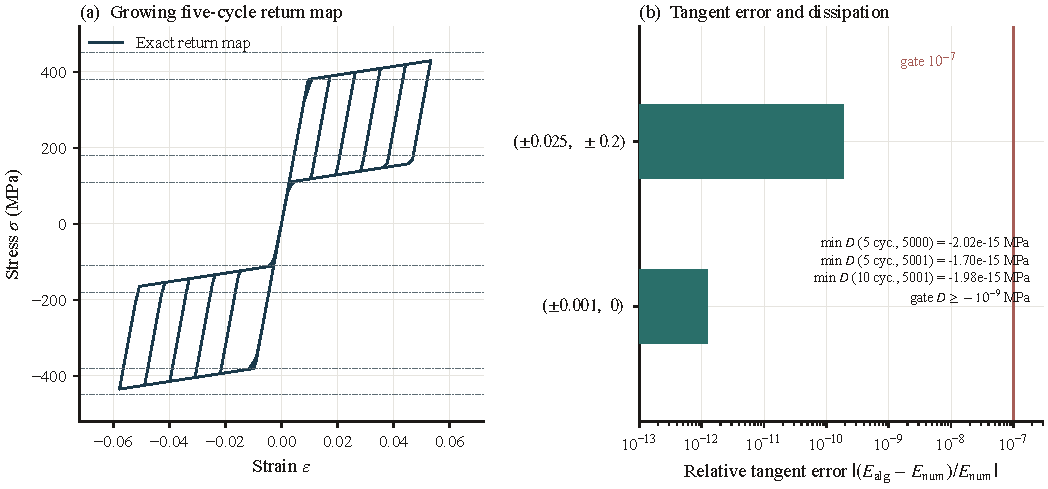
\includegraphics[width=\linewidth]{figures/fig1_constitutive_verification.pdf}
  \caption{Constitutive verification. (a) Exact return map on a growing five-cycle history. (b) Relative algorithmic-tangent error at the audited states. The vertical line is the $10^{-7}$ gate. The dissipation minima printed on the panel are the $0.05\sin\phi$ checks of \cref{sec:diss}.}
  \label{fig:const}
\end{figure}

\section{Inverse parameter identification under measurement noise}
\label{sec:inverse}

The six targets are the default parameters of \cref{sec:params}. The strain history has 601 samples,
\begin{equation}
  \phi\in[0,1],
  \qquad
  \varepsilon(\phi)=0.06\,(0.25+0.75\phi)\,\sin(10\pi\phi).
\end{equation}
The amplitude grows from 1.5\% to 6\% over five cycles. Stress observations are the exact return map plus Gaussian noise of scale
\begin{equation}
  s_{\mathrm{noise}}=0.03\,\max|\sigma_{\mathrm{true}}|=13.041~\mathrm{MPa},
\end{equation}
drawn with seed 42. The noise fraction stored with the run is 0.03.

The training model is not that return map. It is a differentiable stand-in, \texttt{smooth\_stress\_history}, implemented in PyTorch \cite{paszke2019}: hyperbolic-tangent signs, softplus driving forces, and sigmoid gates, with a transition width of 0.5~MPa. The optimiser sees an internal vector $(E,\sigma_{Ms},H_f,\sigma_{Af},H_r,\varepsilon_L)$. A sigmoid maps an unconstrained logit into the bounds $E\in[20000,60000]$~MPa, $\sigma_{Ms}\in[250,500]$~MPa, $H_f\in[20,150]$~MPa, $\sigma_{Af}\in[50,200]$~MPa, $H_r\in[20,150]$~MPa, and $\varepsilon_L\in[0.03,0.09]$. Then $\sigma_{Mf}=\sigma_{Ms}+H_f$ and $\sigma_{As}=\sigma_{Af}+H_r$. The start point $(38000,\,360,\,80,\,120,\,80,\,0.058)$ decodes to $\sigma_{Mf}=440$~MPa and $\sigma_{As}=200$~MPa. After each Adam step the unconstrained parameters are clamped to $[-8,8]$.

Twenty residual-bootstrap curves are stacked with the original noisy curve, giving 21 curves. Residuals are resampled with replacement from the original noise. One shared loss trains all 21 rows,
\begin{equation}
  \label{eq:loss}
  \mathcal{L}
  =\mathrm{mean}\Biggl(
    \Biggl(\frac{\sigma_{\mathrm{smooth}}(\varepsilon;\theta_b)-\sigma_{\mathrm{obs},b}}{s}\Biggr)^{\!2}
  \Biggr),
  \qquad
  s=\max|\sigma_{\mathrm{obs}}|.
\end{equation}
The arithmetic is float64 on one CPU thread. Adam runs for 300 steps at learning rate 0.04. L-BFGS then runs with $\texttt{max\_iter}=80$, history size 20, gradient tolerance $10^{-9}$, change tolerance $10^{-12}$, and a strong Wolfe line search. The reported point is row 0. The 95\% intervals are the 2.5 and 97.5 percentiles of rows 1 to 20 only. After the fit, the stress curve in \cref{fig:inverse} is recomputed with the exact return map at the recovered parameters. The loss itself never sees that exact map.

\Cref{tab:inverse} gives the recovery. Relative error is $|\hat\theta/\theta-1|\times 100$. Every parameter is inside 8\%. The stresses $\sigma_{Ms}$ and $\sigma_{Mf}$ are recovered to about 0.5\%. $\sigma_{As}$ misses by 3.58\%, and $\varepsilon_L$ is the worst case at 7.28\%, moving from 0.06 to 0.06437. The outer loop in \cref{fig:inverse}a still closes on the noisy observations. The flag width and the plateau stresses are the easier features. The transformation strain, which sets how far the plateau runs, is the soft one.

\begin{table}[t]
  \centering
  \small
  \setlength{\tabcolsep}{4.5pt}
  \caption{Recovered parameters under 3\% stress noise. Relative error is $|\hat\theta/\theta-1|\times 100$. The true column is the default set in \cref{sec:params}.}
  \label{tab:inverse}
  % Source: data/diff_id_uncertainty.json. Relative error is |theta_hat/theta - 1| x 100.
\begin{tabular}{llrrrl}
\toprule
Symbol & Meaning & True & Recovered & Error (\%) & Unit \\
\midrule
$E$ & Young modulus & 40000 & 39834.22 & 0.414 & MPa \\
$\sigma_{Ms}$ & Martensite start stress & 380 & 381.74 & 0.458 & MPa \\
$\sigma_{Mf}$ & Martensite finish stress & 450 & 452.17 & 0.483 & MPa \\
$\sigma_{As}$ & Austenite start stress & 180 & 186.45 & 3.582 & MPa \\
$\sigma_{Af}$ & Austenite finish stress & 110 & 111.72 & 1.562 & MPa \\
$\varepsilon_L$ & Transformation strain & 0.06 & 0.06437 & 7.282 & 1 \\
\bottomrule
\end{tabular}

\end{table}

Coverage is a separate fact, and it fails. The 95\% intervals are approximately $[39385,\,40482]$~MPa for $E$, $[378.16,\,380.83]$~MPa for $\sigma_{Ms}$, $[450.85,\,457.82]$~MPa for $\sigma_{Mf}$, $[171.09,\,183.82]$~MPa for $\sigma_{As}$, $[110.64,\,117.14]$~MPa for $\sigma_{Af}$, and $[0.0627,\,0.0658]$ for $\varepsilon_L$. The interval excludes the true $\sigma_{Mf}=450$~MPa, the true $\sigma_{Af}=110$~MPa, and the true $\varepsilon_L=0.06$. It also excludes the recovered $\sigma_{Ms}$ and the recovered $\sigma_{As}$. Twenty bootstrap members are a small sample, and a percentile interval of that size is not a calibrated confidence set. The pointwise 8\% gate can pass while the interval misses the truth. Both statements belong next to \cref{tab:inverse}.

\begin{figure}[t]
  \centering
  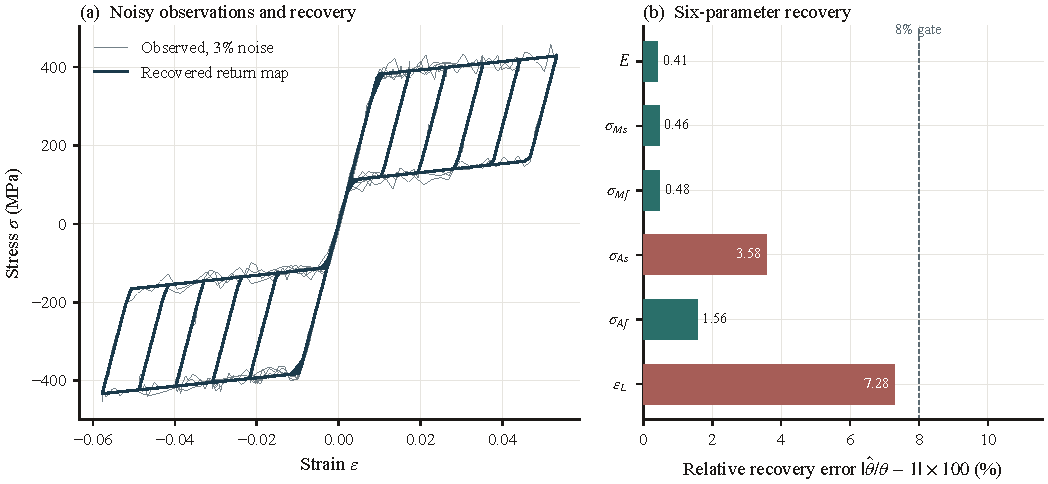
\includegraphics[width=\linewidth]{figures/fig2_inverse_id.pdf}
  \caption{Inverse identification. (a) Observations at 3\% noise, and the exact return map at the recovered parameters. (b) Relative error $|\hat\theta/\theta-1|\times 100$. The dashed line is the 8\% gate. Numerical labels match \cref{tab:inverse} to the printed precision.}
  \label{fig:inverse}
\end{figure}

\section{Diagrid seismic benchmark and surrogate-assisted screening}
\label{sec:frame}

\subsection{Structural model}
\label{sec:ideal}

The canopy is a five-parameter family. Span $L$ lies in $[14,28]$~m, the arch rise in $[0.08L,\,0.22L]$, the number of roof divisions $n_x$ is an even integer in $\{6,8,10,12\}$, the glulam depth lies in $[0.22,0.48]$~m, and the NiTi fuse area lies in $[60,260]$~mm$^2$. The plan width is $0.5L$. A stored branch-spread ratio does not move a node. The roof surface, with a clear-height constant of 4.5~m, is
\begin{equation}
  \label{eq:roof}
  y(x,z)=4.5+\mathrm{arch\_rise}\,
  \bigl(1-(2x/L)^2\bigr)\,
  \bigl(1-0.5\,(2z/\mathrm{width})^2\bigr).
\end{equation}
Four steel trunks rise from $(\pm 0.32L,\,0,\,\pm 0.25\,\mathrm{width})$ to a bifurcation at $y=2.475$~m. Branches run from each bifurcation to the four nearest roof nodes. The diagrid is both diagonals of every roof cell. Steel edge members close the perimeter. Each column has two fuse bars from the bifurcation to ground anchors 1.5~m either side of the column. A six-division canopy has 51 nodes.

The analysis is OpenSeesPy 3.8.0.0, three-dimensional, six degrees of freedom per node \cite{zhu2018,mckenna2011}. Glulam, edge steel, trunks, and branches are elastic beam-column elements with a linear geometric transformation. There are no fibre sections and no $P$-$\Delta$ transformation. Glulam uses $E=12.6$~GPa, $G=0.65$~GPa, density 420~kg/m$^3$, width 0.16~m, and a utilisation stress of 18~MPa. Steel members use $E=210$~GPa, $G=81$~GPa, density 7850~kg/m$^3$, and $f_y=355$~MPa. Edge, trunk, and branch areas are $9.49\times 10^{-3}$, $1.22\times 10^{-2}$, and $4.67\times 10^{-3}$~m$^2$. Trunk bases release torsion about global $Z$. Fuse anchors are fixed.

The time-history model does not call the return map of \cref{sec:return}. NiTi fuses are the OpenSees flag-shaped \texttt{SelfCentering} material, area $A_{\mathrm{NiTi}}\times 10^{-6}$~m$^2$, density 6450~kg/m$^3$. The initial stiffness is $k_1=40$~GPa. The post-activation stiffness is the transformation tangent of \eqref{eq:tangent} converted to pascals,
\begin{equation}
  k_2=1.133603\times 10^{9}~\mathrm{Pa}.
\end{equation}
Activation is $\sigma_{\mathrm{act}}=380$~MPa and the flag parameter is $\beta=(380-110)/380=0.7105$. Slip strain is zero, the bearing strain is 0.071, and the bearing ratio is 1. The bearing strain is not $\varepsilon_L=0.06$. That mismatch is in the model that was run.

The steel fuse is \texttt{Steel02}, sized for equal activation force rather than equal stiffness or equal base shear,
\begin{equation}
  A_{\mathrm{steel}}=(380/355)\,A_{\mathrm{NiTi}}=1.0704\,A_{\mathrm{NiTi}}.
\end{equation}
Its parameters are $f_y=355$~MPa, $E_0=200$~GPa, hardening ratio $b=0.01$, $R_0=18$, $c_{R1}=0.925$, $c_{R2}=0.15$, and density 7850~kg/m$^3$. Because $355 A_{\mathrm{steel}}=380 A_{\mathrm{NiTi}}$, the two fuses activate at the same axial force. They do not have the same $EA$.

Gravity is $g=9.80665$~m/s$^2$. Roof dead load is $G=1.50$~kN/m$^2$, live load $Q=0.75$~kN/m$^2$, and wind uplift $W=1.20$~kN/m$^2$. Static combinations, on separate models, are $1.35G+1.50Q$ and $0.90G+1.50W$, with member self-weight included. These factors are the combinations implemented in the model. The audited record does not tie them to a numbered code clause. Equilibrium error on the 80-design set stays at or below $9.37\times 10^{-11}$ for steel and $3.45\times 10^{-11}$ for NiTi.

Seismic preload is $1.0G$ including self-weight. Seismic mass is roof dead load plus member mass. Live load is not in the mass. Rotational masses are $10^{-3}$. Rayleigh damping is 5\% of modes 1 and 2. The excitation is uniform in global $X$ only. The integrator is Newmark with $\gamma=0.5$ and $\beta=0.25$, time step 0.01~s, and a displacement-increment tolerance of $10^{-8}$.

Roof drift is $\max|u_x|$ over roof nodes, divided by the fixed 4.5~m. It is not divided by the local roof height. Permanent residual drift is the absolute value of the mean signed roof drift over the last 1.0~s.

\subsection{Ground motion and carbon rules}

Each record is a sum of 48 sinusoids. Frequencies are spaced geometrically from 0.35~Hz to 18~Hz, amplitudes scale as $1/\sqrt{f}$, and phases come from the seed. An envelope rises with time constant 0.65~s and decays after 9~s. The 12~s strong motion is scaled to the requested peak, here $0.40g$, and 6~s of zeros follow: 1801 samples and 1800 analysis steps. The generator does not match a code spectrum. The 80-design table and the certified fronts use seed 101 only. Two further seeds exist in the test file. Their means were not saved, and they are not quoted here.

Carbon is a cradle-to-gate factor table plus one design-earthquake repair rule. Biogenic carbon is off. Glulam is 0.512~kgCO$_2$e/kg, steel including the steel fuse is 1.55~kgCO$_2$e/kg, and NiTi is 28.0~kgCO$_2$e/kg. Concrete footings are a fixed 1612.8~kgCO$_2$e. Mass uses the section areas of the analysis model. Modules A1--A3 are the footing term plus the superstructure. Glazing and connections, at 45~kgCO$_2$e/m$^2$ of shaded area, appear only as repair.

After the design earthquake, a steel fuse is replaced, at 1.5 times its own A1--A3 carbon, if its peak strain exceeds 0.00355. A NiTi fuse is replaced on the same factor if its peak strain exceeds 0.06. At the threshold, replacement is zero. The glazing ratio is zero at peak drift of 0.5\% or less, rises linearly to the start of a cap at 2.5\% drift, and is 0.60 above 2.5\%. Residual repair is $\min(1,\,d_{\mathrm{res}}/0.005)$ times 40\% of the superstructure carbon. Footings sit outside that base. Lifecycle intensity divides A1--A3 plus repair by the shaded area. Transport, construction, and end of life are absent.

\subsection{Paired comparison at \texorpdfstring{$0.40g$}{0.40 g}}

The sample is an 80-row Latin hypercube, seed 42, with 20 designs in each division count. Span runs from 14.05~m to 27.86~m. Every row passed 1800 steps and the static equilibrium gate. \Cref{tab:compare} is the comparison. Counts below are on the same 80 geometries.

\begin{table}[t]
  \centering
  \small
  \setlength{\tabcolsep}{6pt}
  \caption{Means over 80 paired canopies, ground-motion seed 101, peak acceleration $0.40g$. Drift quantities are in percent. False-safe rates are fractions of the 80 designs of that fuse. The $R^2$ row is grouped cross-validation for peak drift.}
  \label{tab:compare}
  % Means from data/verified_lhs_dataset.csv (80 paired designs, seed 101, 0.40 g).
% Screening rates from data/gp_surrogate.json validation.per_case.
\begin{tabular}{lrrl}
\toprule
Quantity & Yielding steel & NiTi & Unit \\
\midrule
Peak roof drift, mean & 1.788 & 3.397 & \% \\
Absolute residual drift, mean & 0.0659 & 0.0175 & \% \\
Lifecycle intensity, mean & 174.76 & 184.24 & kgCO$_2$e/m$^2$ \\
A1--A3 carbon, mean & 17669.4 & 18290.3 & kgCO$_2$e \\
False-safe rate, mean rule & 0.050 & 0.050 & fraction of 80 \\
False-safe rate, 95\% UCB & 0.000 & 0.000 & fraction of 80 \\
Peak-drift grouped-CV $R^2$ & 0.379 & 0.808 & -- \\
\bottomrule
\end{tabular}

\end{table}

NiTi peak drift is higher on 80 of 80 designs. The ratio of the unrounded means is 1.90. Medians are 1.530\% for steel and 2.664\% for NiTi, so the ordering is not one outlier. Designs above 2\% peak drift number 17 for steel and 55 for NiTi. Absolute residual drift is lower for NiTi on 66 of 80 designs. The ratio of mean residuals is 0.265. The ratio of median residuals is 0.102, so a typical design recenters by more than the mean ratio suggests. Mean peak base shear is 285.3~kN for steel and 415.3~kN for NiTi, a ratio of 1.46. The equal-force fuse does not produce equal base shear.

Mean A1--A3 carbon is higher for NiTi on 80 of 80 designs, by 620.9~kgCO$_2$e. Mean lifecycle intensity is 174.76~kgCO$_2$e/m$^2$ for steel and 184.24~kgCO$_2$e/m$^2$ for NiTi. The unrounded means differ by 9.475~kgCO$_2$e/m$^2$. Intensity is higher for NiTi on 66 designs and lower on 14. Mean repair is 2875.7~kgCO$_2$e for NiTi and 2435.3~kgCO$_2$e for steel, even though the replacement rule triggers on 1 of 80 NiTi fuses and on 53 of 80 steel fuses. The saved totals do not split repair into fuse, glazing, and residual. The rules leave the drift-linked glazing term as the piece that can raise NiTi repair while NiTi avoids most fuse replacements and has the smaller residual. \Cref{fig:seismic} is the paired cloud.

\begin{figure}[t]
  \centering
  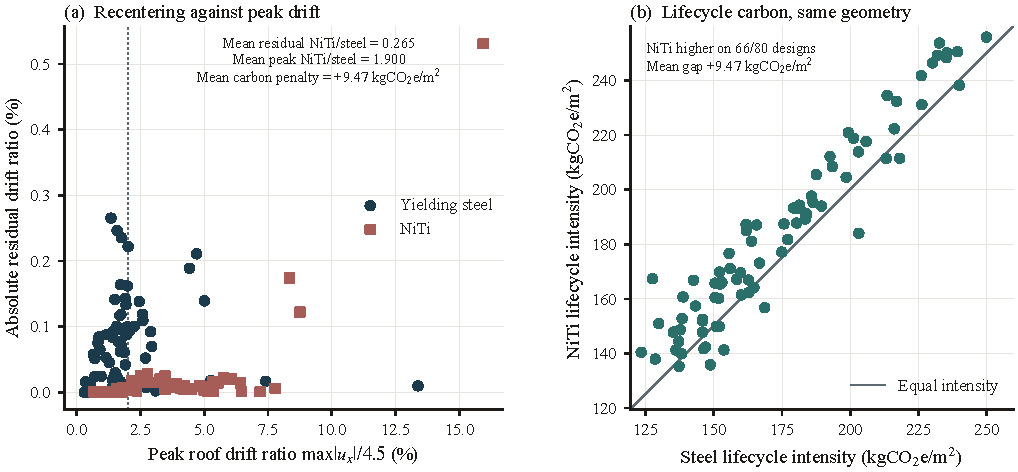
\includegraphics[width=\linewidth]{figures/fig3_seismic_pareto.pdf}
  \caption{Paired $0.40g$ sample, 80 geometries. (a) Absolute residual drift against peak roof drift, $\max|u_x|/4.5$. The annotations are the ratio of mean residuals (0.265), the ratio of mean peak drifts (1.900), and the mean lifecycle gap. (b) Lifecycle intensity on the same geometries. Points above the line are a NiTi penalty. NiTi is higher on 66 of 80 designs.}
  \label{fig:seismic}
\end{figure}

Three of the 80 steel analyses have a fundamental period above 1.50~s. The maximum is 1.722~s. No NiTi analysis in the set exceeds 1.50~s. The maximum NiTi period is 1.447~s. The dataset keeps the three long steel periods.

\subsection{Grouped-CV Gaussian process and NSGA-II}
\label{sec:screen}

Separate Gaussian processes are fit for each fuse \cite{rasmussen2006}. The five features are span, arch-rise ratio, diagrid divisions, glulam depth, and NiTi fuse area. The four targets are peak drift in percent, absolute residual drift in percent, static gravity deflection in millimetres, and lifecycle intensity. The kernel is a constant times a Mat\'ern kernel of smoothness $\nu=2.5$, plus a white-noise kernel. Features are standardised inside each fold and again on the full fit. Cross-validation is four folds grouped by span quartile, 20 rows in each fold.

A held-out row is unsafe when the true peak drift exceeds 2\%. It is false-safe when it is unsafe and the predictor still calls it safe. The mean rule calls a row safe at a predictive mean of 2\% or less. The 95\% upper-confidence rule calls it safe only when the mean plus $1.96$ standard deviations is still at or below 2\%. Pooled over 160 held-out rows (80 designs, two fuses), 72 are unsafe. The mean rule is false-safe on 8 of 160 rows, a rate of 0.050. The upper-confidence rule is false-safe on none. Per fuse the mean rate is 4 of 80 and the upper-confidence count is zero (\cref{fig:gp}, \cref{tab:compare}).

Peak-drift $R^2$ is 0.379 for steel and 0.808 for NiTi. Gravity-deflection $R^2$ is 0.772 and 0.808. Lifecycle-intensity $R^2$ is 0.823 and 0.868. The NiTi residual model has $R^2=-0.154$. A residual objective would not be supported by the surrogate that was trained. The screen therefore constrains peak drift and gravity deflection, and it does not constrain residual drift.

\begin{figure}[t]
  \centering
  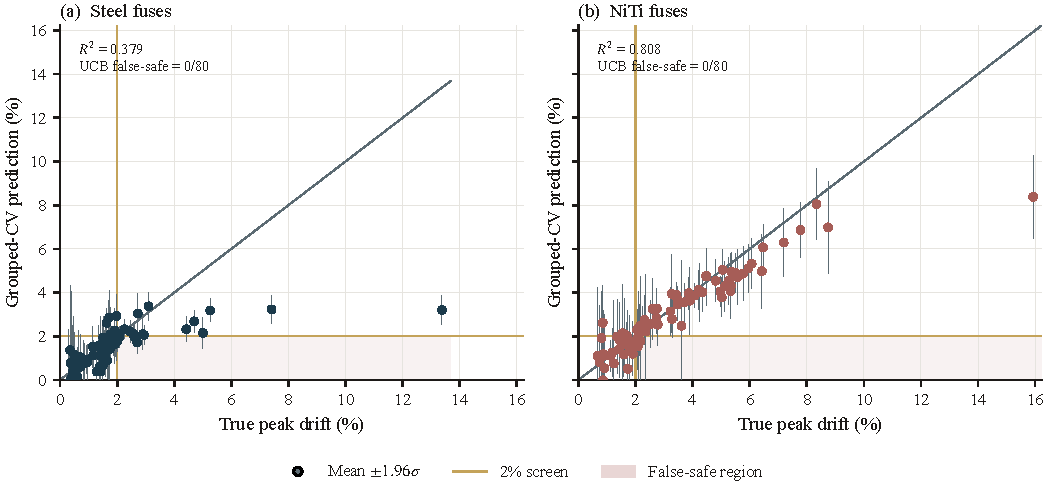
\includegraphics[width=\linewidth]{figures/fig4_gp_screening.pdf}
  \caption{Grouped four-fold peak-drift predictions. (a) Steel, $R^2=0.379$. (b) NiTi, $R^2=0.808$. Bars are the predictive mean plus and minus $1.96$ standard deviations. The shaded band is the region in which a mean at or below 2\% would call an unsafe row safe. The 95\% upper-confidence rule has zero false-safe calls in each panel.}
  \label{fig:gp}
\end{figure}

NSGA-II \cite{deb2002} minimises predicted lifecycle intensity and maximises span, with population 60, 60 generations, and seed 42, once per fuse. Divisions snap to $\{6,8,10,12\}$. Both of the following must be non-positive: the upper confidence bound on peak drift, minus 2\%, and the upper confidence bound on gravity deflection, minus $L/250$. Each accepted point is reanalysed with the exact static cases and the $0.40g$ seed-101 record. A point is rejected if the exact peak drift exceeds 2\% or the exact gravity deflection exceeds $L/250$.

The artifact records 8 attempts, 8 accepted, 0 rejected, and 0 failed analyses: four designs on the steel front and four on the NiTi front. They form two tight clusters, all with six divisions. They do not trace a long curve in carbon and span. Steel-front spans run from 27.20~m to 27.29~m. NiTi-front spans run from 21.20~m to 21.32~m. On the steel-front geometries, switching the fuse to NiTi raises the exact peak drift to about 4.1\% to 4.2\%, so those geometries fail the 2\% gate under NiTi. On the NiTi front the certified NiTi peak drifts run from 1.54\% to 1.82\%. On all eight geometries the NiTi peak drift, peak base shear, A1--A3 carbon, and lifecycle intensity are higher, and the NiTi absolute residual is lower. The constraint, not a spread of trade-off weights, is what separates the two spans. NiTi drifts are larger, so the designs that still clear 2\% are the shorter ones.

\section{Discussion: the recentering, drift, and carbon trade-off}
\label{sec:discuss}

Rounded to two decimal places, the mean peak roof drifts are 3.40\% for NiTi and 1.79\% for steel. \Cref{tab:compare} gives the means before that rounding, 3.397\% and 1.788\%. The ratio of the unrounded means is 1.90, and the inequality holds on every one of the 80 geometries.

The paired designs share the geometry, the mass, and the ground motion. They do not share fuse stiffness. The steel area is set so that the yield force matches the NiTi activation force, and that area is 1.070 times the NiTi area. The NiTi flag starts at 40~GPa. The steel fuse starts at 200~GPa. Elastic axial stiffness scales as $EA$, so the steel fuse is $(200/40)\times 1.070=5.35$ times as stiff as the NiTi fuse before either one activates. After activation the gap remains. The NiTi transformation stiffness is $k_2=1.134$~GPa. The steel hardening modulus is $b E_0=2.0$~GPa, on the larger area. The NiTi fuse stretches further. The mean of the peak fuse strains is 1.550\% for NiTi and 0.758\% for steel. Roof drift, which is the largest roof $|u_x|$ divided by the fixed 4.5~m, follows that stretch.

The larger drift is not a smaller force. Mean peak base shear rises from 285.3~kN to 415.3~kN. Members other than the fuses stay linear elastic, and their geometric transformation is linear, so they do not yield in order to cap the roof displacement. The extra drift is carried by the corotational fuse and by elastic flexure. Median peak drifts are 2.664\% and 1.530\%. The mean ratio is not an artefact of a single record spike on one canopy, though \cref{fig:seismic} does show a long right-hand tail, and 55 NiTi designs exceed 2\% against 17 steel designs.

The recentering result is real on the same rows. Mean absolute residual drift falls from 0.0659\% to 0.0175\%, a ratio of 0.265, and it falls on 66 of 80 designs. The median ratio is 0.102. In the return map this happens because a reverse branch can clear $z$, and because nothing in the model accumulates residual transformation strain from cycle to cycle. DesRoches, McCormick, and Delemont measured degradation of recentering once cyclic strains passed 6\% \cite{desroches2004}. The transformation strain here is 0.06, and the constitutive update has no fatigue variable. Recentering cannot wear out inside the calculation that produced \cref{fig:seismic}.

The carbon penalty is also real, and it is smaller at building scale than the factor ratio suggests. NiTi at 28.0~kgCO$_2$e/kg against steel at 1.55~kgCO$_2$e/kg is a large unit price. The mean A1--A3 total only rises by 620.9~kgCO$_2$e, which is 3.5\% of the steel mean (17669.4~kgCO$_2$e), and it rises on all 80 pairs. The fuse is a small mass next to the glulam diagrid, the steel members, and a fixed footing term of 1612.8~kgCO$_2$e. Lifecycle intensity still rises on 66 of 80 designs, by 9.475~kgCO$_2$e/m$^2$ on the mean, and it falls on the other 14. Mean repair rises even while NiTi fuse replacement almost disappears (1 of 80, against 53 of 80 for steel). The glazing rule is the term in the inventory that grows when peak drift grows. The saved table does not isolate that term, so the split is an inference from the rules and the counts, not a third measured column.

The surrogate can police the drift limit and cannot price the recentering. With the 95\% upper-confidence rule, no held-out row with true peak drift above 2\% is called safe. The steel peak-drift $R^2$ of 0.379 is the weak model of the four screening targets. Gravity and carbon sit between 0.77 and 0.87. The NiTi residual $R^2$ of $-0.154$ means a search that treated residual drift as a predicted objective would be fitting noise. The certified fronts are consistent with that narrow use. Eight exact reanalyses pass, and they collapse to two spans, about 27.2~m in steel and about 21.3~m in NiTi, all with six divisions. Maximising span under a 2\% drift bound pushes each fuse case to the longest span that still clears the bound. It does not draw a curve of carbon against recentering.

\subsection{What the model cannot say}

Four limits decide how far \cref{tab:compare} can be taken.

The constitutive law is one-dimensional, isothermal, and rate-independent. There is no latent heat, no thermal boundary layer, and no cyclic degradation. The discrete check \eqref{eq:diss} passed on the sine histories that were audited. It is not a derivation of the flow rule, and it says nothing about a transformation front with a temperature field.

The frame does not integrate that law. The NiTi fuse is a flag-shaped uniaxial material whose bearing strain, 0.071, is not the transformation strain 0.06. Every other member is linear elastic. The geometric transformation on those members is linear. The ground motion is one horizontal component. Drift divides roof displacement by a fixed 4.5~m, so a tall arch and a flat arch are scored on the same denominator. A uniform bar strain cannot represent a transformation front along a short fuse, and it cannot represent multiaxial stress at the bifurcation.

The hazard is one synthetic waveform at $0.40g$, seed 101. There is no recorded suite and no target spectrum. A period band of 0.15~s to 1.50~s is not enforced on the 80-row set. Three steel periods lie above 1.50~s and remain in the means.

The carbon boundary stops at modules A1--A3 plus repair from a single design earthquake. A biogenic glulam factor of $-0.98$~kgCO$_2$e/kg exists in the code and is switched off in the numbers above. Turning it on would change the glulam term for both fuses alike. It would not, by itself, remove the NiTi unit price.

These limits point in one direction. The missing physics is a three-dimensional thermomechanical constitutive model: temperature, latent heat, and a transformation strain that can vary through a section and along a bar. The missing kinematics, for a fuse short enough that the transformation is a front rather than a uniform strain, is an enriched continuum with a length tied to that front. The present paper stops at the uniform isothermal bar, and at a frame that never calls it. The drift and carbon penalties in \cref{tab:compare} are the reason that stop matters. They are properties of this idealisation, on this sample.

Two smaller facts belong with those limits. The branch-spread parameter does not move a node, so one coordinate of the design vector is inert. The 20-member identification intervals miss the true transformation strain. A downstream study that treated $\varepsilon_L=0.06437$ as known, or that treated a branch-spread ratio as a built dimension, would be using a number the present evidence does not support.

\section{Conclusion and reproducibility}
\label{sec:close}

On this sample, superelastic NiTi does recenter the roof and does not improve the other two scores. Mean absolute residual drift falls from 0.0659\% to 0.0175\%. Mean peak drift rises from 1.79\% to 3.40\% on all 80 geometries, because the equal-force fuse is several times softer than the steel fuse it replaces, in both the elastic branch and the post-activation branch. Mean cradle-to-gate carbon rises by 620.9~kgCO$_2$e, and lifecycle intensity rises on 66 of 80 designs. The return map that supplied the fuse stresses passes its tangent gate at $1.85\times 10^{-10}$ and its dissipation gate of $-10^{-9}$~MPa. The identification recovers every parameter to within 8\% under 3\% stress noise, and its bootstrap intervals miss three true values. The grouped-CV screen can hold a 2\% drift limit with an upper-confidence false-safe rate of zero. The certified fronts collapse to two spans.

The repository is \url{https://github.com/syednafizreja/diagrid-seismic-opt}, commit \texttt{85a698c} on \texttt{main}. The audit date of the numbers in this preprint is 26~November 2026. OpenSeesPy is 3.8.0.0. The identification used PyTorch in float64 on one CPU thread, Adam at learning rate 0.04 for 300 steps, then L-BFGS with iteration limit 80, history size 20, gradient tolerance $10^{-9}$, change tolerance $10^{-12}$, and a strong Wolfe line search \cite{paszke2019}. NSGA-II used population 60, 60 generations, and seed 42 \cite{deb2002}. The audited fact sheet does not record the PyTorch, pymoo, or scikit-learn version strings. Seeds that are recorded are 42 for the identification noise, the Latin hypercube, and the surrogate and search, and 101 for the published ground motion.

The test file contains 25 test functions. Three of them are parametrised over steel and NiTi, so a collection is 28 tests. Five functions are constitutive. This audit recomputed the dissipation minima and the tangent errors in \cref{sec:diss,sec:tangent}. Both gates pass. The Newton residual at 500~MPa is $4.547\times 10^{-13}$. The audit did not execute the test runner, so this paper does not claim a fresh pass of the full suite. The paired means are the saved 80-row table. The time histories and the identification fit were not repeated for this preprint.

\bibliographystyle{unsrt}
\bibliography{refs}

\end{document}
